\documentclass{article}
\usepackage{iclr2027_conference,times}
\usepackage[T1]{fontenc}
\usepackage[utf8]{inputenc}
\usepackage{microtype}
\usepackage{amsmath,amssymb,amsthm}
\usepackage{graphicx,booktabs,tabularx}
\usepackage{algorithm,algpseudocode}
\usepackage{subcaption}
\usepackage{placeins}
\usepackage{xurl}
\usepackage{hyperref}
\usepackage[capitalize,noabbrev]{cleveref}
\usepackage{xspace}

\newcommand{\ours}{REINFORCE++\xspace}
\newcommand{\baseline}{REINFORCE++-Baseline\xspace}
\newcommand{\E}{\mathbb{E}}
\newcommand{\KL}{D_{\mathrm{KL}}}
\newcommand{\sg}{\operatorname{sg}}
\newtheorem{proposition}{Proposition}
\newtheorem{remark}{Remark}
\hypersetup{pdftitle={REINFORCE++: Stabilizing Critic-Free Policy Optimization with Global Normalization},pdfauthor={},pdfsubject={Anonymous ICLR 2027 submission},pdfkeywords={reinforcement learning, RLHF, policy optimization, advantage normalization}}

\title{REINFORCE++: Stabilizing Critic-Free Policy\\Optimization with Global Normalization}
\author{Anonymous authors}
% Keep \iclrfinalcopy disabled for double-blind submission.

\begin{document}
\maketitle
\begin{abstract}
Critic-free reinforcement learning reduces the cost of post-training large language models, but its behavior depends strongly on how rewards are converted into advantages. In group-relative methods, normalizing rewards separately for each prompt couples the update scale to statistics estimated from a small set of responses. We introduce REINFORCE++, a critic-free policy optimization framework that instead normalizes advantages across the rollout batch. The basic variant supports one or more responses per prompt and incorporates a token-level KL penalty into Monte Carlo returns. A second variant, REINFORCE++-Baseline, combines a within-prompt reward baseline with global normalization and a separate KL regularizer. Our analysis characterizes finite-sample normalization and its convergence to population standardization under independent sampling. Experiments cover preference-based alignment, mathematical and logical reasoning, and multi-step tool use. With one response per prompt, REINFORCE++ obtains an Arena-Hard score of 46.7, compared with 46.8 for four-response GRPO. In tool-use experiments, REINFORCE++-Baseline achieves an average score of 24.10, compared with 22.58 for GRPO and 21.85 for PPO. These results support global normalization as a practical design choice for critic-free language-model training.
\end{abstract}

\section{Introduction}
Reinforcement learning (RL) is a central component of language-model post-training. It can optimize models against learned human-preference rewards~\citep{Ouyang2022} or verifiable task outcomes~\citep{shao2024deepseekmath,guo2025deepseek}. Proximal policy optimization (PPO; \citealp{schulman2017proximal}) provides a widely used training objective, but its actor--critic implementation requires a value model in addition to the policy. Training and storing this critic increases the resource requirements of large-model alignment.

Critic-free methods avoid this extra model by estimating advantages directly from sampled rewards. ReMax uses a greedy response as a baseline~\citep{li2023remax}, RLOO uses a leave-one-out baseline~\citep{2024Back}, and group relative policy optimization (GRPO) standardizes rewards within each prompt's response group~\citep{shao2024deepseekmath}. These methods differ in both their baselines and their normalization rules. In particular, RLOO does not inherently require the group-standard-deviation normalization used by GRPO.

This paper focuses on the \emph{scope of advantage normalization}. A prompt-level standard deviation is estimated from only a few responses and introduces a separate scale for every prompt. As a result, the update depends on the composition of each sampled group, as well as on its rewards. Homogeneous groups contribute no centered reward signal, whereas groups with different reward spreads are rescaled independently. These effects motivate separating two decisions: whether to use a prompt-specific baseline and whether to use a prompt-specific scale.

We introduce \ours, a critic-free framework that uses a shared normalization across the rollout batch. The basic variant combines Monte Carlo returns with PPO clipping and supports $k\geq 1$ responses per prompt. At $k=1$, it allocates each rollout to a different prompt. The \baseline variant retains a within-prompt mean baseline for $k>1$, then normalizes globally and applies a separate KL regularizer. This distinction preserves the option of comparing responses to the same prompt without assigning each prompt its own standard-deviation scale.

Our contributions are threefold. First, we specify both variants within a common clipped policy objective, including the loss reduction used in our experiments. Second, we characterize the finite-sample effects of self-normalization and establish convergence to population standardization under independent sampling. Third, we evaluate the methods across preference-based alignment, reasoning, and tool use. The results show competitive alignment scores with single-response sampling, improved held-out performance in several reasoning settings, and the highest average tool-use score among the compared methods.

\section{Background and related work}\label{sec:background}
\paragraph{Clipped policy optimization.}
Let $q$ be a prompt, $o=(o_1,\ldots,o_T)$ a sampled response, and $h_t=(q,o_{<t})$ its token context. Rollouts are generated by a fixed policy $\pi_{\mathrm{old}}$, and $\pi_\theta$ is the policy being updated. Define the token probability ratio and clipped surrogate as
\begin{align}
 s_t(\theta)&=\frac{\pi_\theta(o_t\mid h_t)}{\pi_{\mathrm{old}}(o_t\mid h_t)},\\
 f_t(\theta,A_t)&=\min\!\left\{s_t(\theta)A_t,\,
 \operatorname{clip}(s_t(\theta),1-\varepsilon,1+\varepsilon)A_t\right\}.
 \label{eq:clipped}
\end{align}
The response-averaged PPO objective is
\begin{equation}
 J_{\mathrm{clip}}(\theta)=\E_{q,\,o\sim\pi_{\mathrm{old}}(\cdot\mid q)}
 \left[\frac{1}{T}\sum_{t=1}^{T}f_t(\theta,A_t)\right].
 \label{eq:ppo}
\end{equation}
PPO commonly obtains $A_t$ from a learned value function using generalized advantage estimation~\citep{schulman2018highdimensionalcontinuouscontrolusing}. Critic-free methods instead construct $A_t$ from observed rewards. All advantages are held fixed while optimizing \cref{eq:ppo}.

\paragraph{Baselines and normalization are separate choices.}
For $k$ responses to the same prompt, write $r_i=r(q,o^{(i)})$, $\bar r_q=k^{-1}\sum_i r_i$, and $s_q^2=k^{-1}\sum_i(r_i-\bar r_q)^2$. ReMax subtracts the reward of a greedy response. RLOO uses
\begin{equation}
 A_i^{\mathrm{RLOO}}=r_i-\frac{1}{k-1}\sum_{j\ne i}r_j,
 \qquad k>1.
 \label{eq:rloo}
\end{equation}
GRPO uses the group-standardized reward
\begin{equation}
 A_i^{\mathrm{GRPO}}=\frac{r_i-\bar r_q}{s_q+\eta},
 \qquad \eta>0.
 \label{eq:grpo}
\end{equation}
Thus, the group mean controls centering, while $s_q$ controls the relative scale of different prompts. Each group receives its own scale, estimated from $k$ responses. Our method retains the option of a group baseline while sharing the normalization scale across the rollout batch. \Cref{appendix:normalization} analyzes the finite-sample behavior of group standardization and its large-sample limit.

\paragraph{Normalization in RL.}
Advantage normalization is an established implementation choice in policy optimization~\citep{andrychowicz2020matters}. Our focus is its use in critic-free language-model training and its interaction with prompt baselines, KL regularization, and response sampling. Related studies examine RL implementation choices~\citep{liu2025part}, compute scaling~\citep{khatri2025art}, and batch-wise normalization in length-constrained reasoning~\citep{liu2025dler}. Together, these studies emphasize the practical importance of normalization and loss design across language-model RL settings.

\section{REINFORCE++}\label{sec:method}
We use a rollout batch $\mathcal B$ containing $B$ sampled responses. With $k$ responses per prompt, the batch contains $B/k$ prompt groups when $B$ is divisible by $k$. We reserve $E$ for the number of optimization epochs, $\varepsilon$ for PPO clipping, and $\eta$ for numerical stabilization.

\subsection{Monte Carlo returns with global normalization}
The basic variant uses the terminal task reward and a token-level log-ratio penalty. For response $i$, define
\begin{align}
 d_{i,t}&=\log\frac{\pi_{\mathrm{old}}(o_{i,t}\mid h_{i,t})}
 {\pi_{\mathrm{ref}}(o_{i,t}\mid h_{i,t})},\\
 G_{i,t}&=r(q_i,o_i)-\beta\sum_{u=t}^{T_i}d_{i,u}.
 \label{eq:return}
\end{align}
Here $\pi_{\mathrm{ref}}$ is a fixed reference policy and $\beta\geq0$. With undiscounted returns, the terminal task reward contributes to every preceding response token. It is the immediate task reward, rather than the return, that is zero before termination.

We center and scale the returns using statistics from the full rollout batch:
\begin{equation}
 \widehat A_{i,t}=\frac{G_{i,t}-\mu_{\mathcal B}}{\sigma_{\mathcal B}+\eta}.
 \label{eq:global}
\end{equation}
The moments are computed over valid response positions, excluding padding. They are shared across prompt groups and held fixed during subsequent minibatch updates. This global normalization is distinct from the reduction of token losses, which averages within each response before averaging across responses (\cref{appendix:batch_mean}).

Pooling observations across prompts makes the normalization depend on the full batch rather than any one small group. It also gives every prompt a common scale during optimization. \Cref{appendix:normalization} characterizes finite-sample normalization and establishes its convergence under independent sampling.

The basic variant maximizes \cref{eq:ppo} with $A_t=\widehat A_t$. It requires neither a critic nor multiple responses to a prompt. The same construction also applies when $k>1$.

\begin{algorithm}[t]
\caption{REINFORCE++ with $k\geq1$ responses per prompt}
\label{algo:main}
\begin{algorithmic}[1]
\Require Policy $\pi_\theta$, reference $\pi_{\mathrm{ref}}$, reward function $r$, prompt data
\Require Rollout size $B$, responses per prompt $k$, optimization epochs $E$
\For{each rollout step}
 \State Freeze $\pi_{\mathrm{old}}\gets\pi_\theta$
 \State Sample $B/k$ prompts and $k$ responses per prompt from $\pi_{\mathrm{old}}$
 \State Evaluate rewards and compute token returns using \cref{eq:return}
 \State Compute global moments and normalized advantages using \cref{eq:global}
 \State Detach advantages and retain old-policy log probabilities
 \For{$e=1,\ldots,E$}
  \For{each response minibatch}
   \State Update $\theta$ with the batch mean loss in \cref{eq:batch_mean}
  \EndFor
 \EndFor
\EndFor
\State \Return $\pi_\theta$
\end{algorithmic}
\end{algorithm}

\subsection{A group-baseline variant}
\label{sec:baseline}
For tasks with multiple responses per prompt, \baseline first subtracts a within-prompt mean reward:
\begin{equation}
 C_{q,i}=r(q,o^{(i)})-\frac{1}{k}\sum_{j=1}^{k}r(q,o^{(j)}),
 \qquad k>1.
 \label{eq:group_center}
\end{equation}
We broadcast $C_{q,i}$ to the valid response tokens and apply the global normalization in \cref{eq:global}, using $C$ in place of $G$. The group baseline removes a shared reward offset for each prompt; global scaling then applies a common scale across the batch.

The group mean includes the current response. In fact,
\begin{equation}
 C_{q,i}=\frac{k-1}{k}A_i^{\mathrm{RLOO}}.
 \label{eq:rloo_relation}
\end{equation}
This identity makes the relation to RLOO explicit. Group centering focuses the reward contrast on groups whose sampled responses have different outcomes.

This variant uses a separate KL regularizer rather than including the KL penalty in \cref{eq:group_center}. Define
\begin{equation}
 z_{i,t}(\theta)=\log\frac{\pi_\theta(o_{i,t}\mid h_{i,t})}{\pi_{\mathrm{ref}}(o_{i,t}\mid h_{i,t})},
 \qquad k_2(z)=\tfrac12 z^2.
\end{equation}
The training loss is
\begin{equation}
 L_{\mathrm{Baseline}}(\theta)=L_{\mathrm{PG}}(\theta)
 +\beta_{\mathrm{KL}}\frac{1}{B}\sum_{i=1}^{B}
 \frac{1}{T_i}\sum_{t=1}^{T_i}\tfrac12 z_{i,t}(\theta)^2,
 \label{eq:baseline_loss}
\end{equation}
where $L_{\mathrm{PG}}$ is the negative clipped surrogate. For a fixed context and on-policy action samples, the expected gradient obtained by differentiating $k_2$ with sampled actions held fixed matches the reverse-KL gradient~\citep{liu2025rethinking}. This is a statement about a gradient surrogate, not equality of KL values or of full sequence objectives. Reusing old-policy rollouts makes the uncorrected estimator off-policy; \cref{appendix:kl} states the distinction precisely.

\subsection{Relationship to PPO and practical cost}
Setting the value function to zero and taking $\gamma=\lambda_{\mathrm{GAE}}=1$ reduces GAE to an undiscounted Monte Carlo return. The basic variant uses this return structure, followed by batch normalization. The group-baseline variant adds prompt-specific reward centering and moves KL regularization into a separate loss. Both retain PPO's clipped surrogate while replacing the learned critic with directly computed reward statistics.

Both variants remove critic training and storage. At fixed response budget $B$, the $k=1$ configuration permits up to $B$ distinct prompts, whereas grouped sampling uses $B/k$. This is a sampling-budget comparison: realized runtime and memory also depend on generation lengths, batching, and the implementation.

\section{Experiments}\label{sec:experiments}
We evaluate preference-based alignment, mathematical and logical reasoning, and multi-step tool use with OpenRLHF~\citep{hu2024openrlhf}. The basic variant is used in the alignment and reasoning experiments; \baseline is used in the tool-use comparison. All reported losses use a mean over valid tokens within each response followed by a mean over responses (\cref{appendix:batch_mean}).

\subsection{Preference-based alignment}\label{sec:alignment}
\paragraph{Setup.}
We train a Llama-3-8B-SFT policy on 20,000 prompts using a Bradley--Terry reward model trained on approximately 700,000 human-preference pairs. We compare \ours with one sampled response per prompt against GRPO and RLOO with four responses per prompt, and ReMax with one sampled and one greedy response. Evaluation uses Arena-Hard~\citep{li2024crowdsourced}.

\begin{table}[htbp]
\caption{Arena-Hard results. Length is the mean generated response length, and score/length is their ratio. REINFORCE++ achieves a competitive score with one sampled response per prompt.}
\label{tab:alignment}
\centering
\begin{tabular}{lrrr}
\toprule
Method & Score & Length & Score/length \\
\midrule
\ours ($k=1$) & 46.7 & 832 & \textbf{0.0561} \\
GRPO ($k=4$) & \textbf{46.8} & 860 & 0.0544 \\
RLOO ($k=4$) & 44.6 & 866 & 0.0515 \\
ReMax (1 sampled + 1 greedy) & 45.1 & \textbf{805} & 0.0560 \\
\bottomrule
\end{tabular}
\end{table}

\paragraph{Results.}
\Cref{tab:alignment} shows that \ours obtains 46.7, close to GRPO's 46.8, while generating shorter responses on average (832 versus 860 tokens). It also has the highest score/length ratio among the compared methods. These results demonstrate competitive preference alignment with one sampled response per prompt, enabling the rollout budget to cover a broader set of prompts.

\begin{figure}[htbp]
\centering
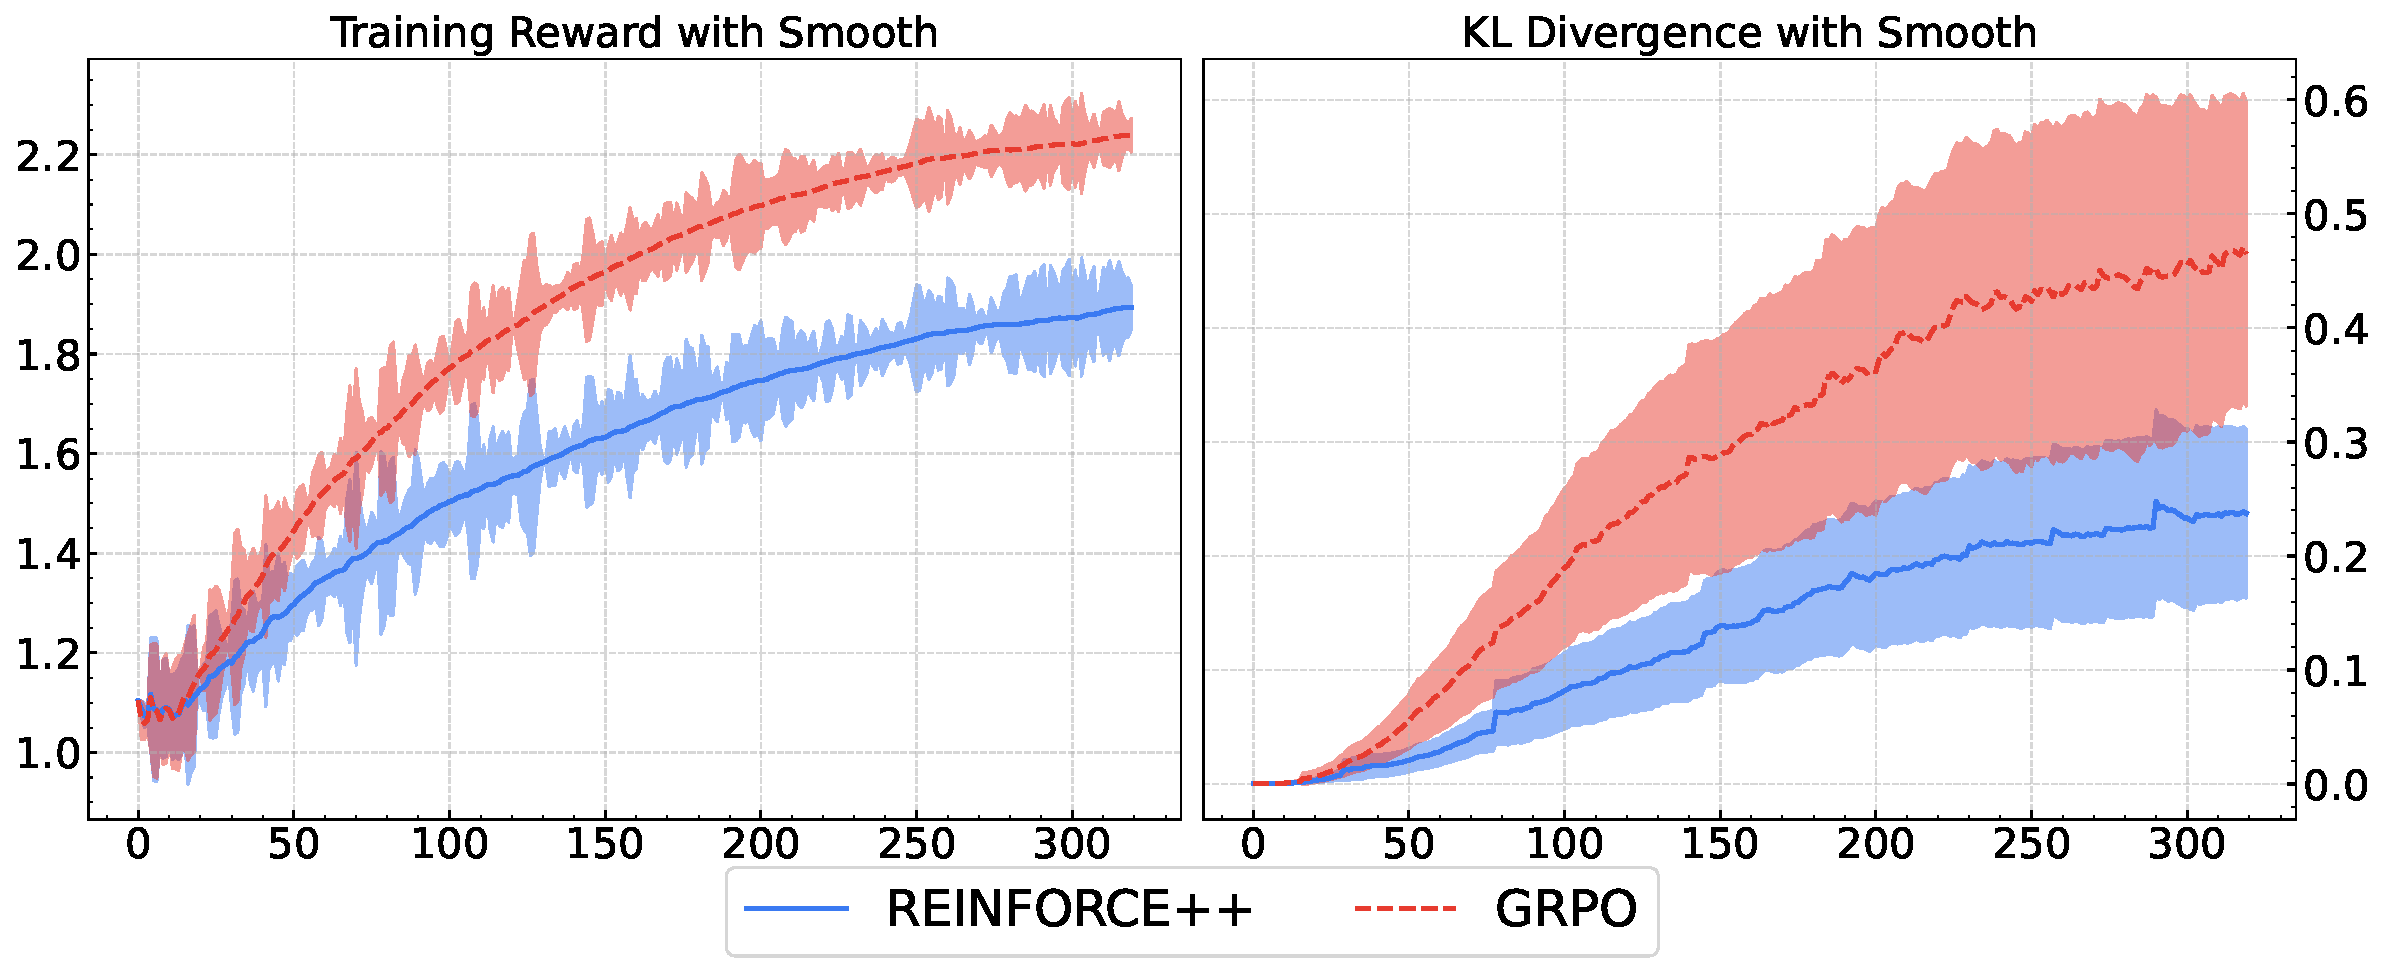
\includegraphics[width=\linewidth]{imgs/orm_reward_kl.pdf}
\caption{Smoothed training reward and KL divergence in preference-based alignment. \ours combines increasing reward with a lower KL divergence throughout the reported training trajectory.}
\label{fig:reward_kl}
\end{figure}

\Cref{fig:reward_kl} shows different reward--KL trade-offs: GRPO's reward rises rapidly alongside its KL divergence, whereas \ours maintains a smaller divergence. This behavior illustrates controlled policy updates under global normalization and KL-regularized returns.

\FloatBarrier
\subsection{Mathematical and logical reasoning}\label{sec:reasoning}
These experiments use the basic \ours variant with grouped sampling ($k>1$) and compare it with GRPO. Mathematical reasoning is trained with verifiable rewards, following the broader RLVR setting~\citep{guo2025deepseek,seed2025seed1}.

\paragraph{Learning from a small prompt set.}
We train on 30 AIME 2024 questions and evaluate on AIME 2025. In \cref{tab:small}, GRPO has the higher training score (95.0 versus 71.0), while \ours has the higher held-out scores: 2.5 versus 0.0 at pass@1 and 40.0 versus 0.4 at pass@16. The comparison highlights the distinction between fitting the training prompts and transferring to a new problem set. In this small-data setting, global normalization is associated with stronger held-out performance.

\begin{table}[htbp]
\caption{Small-data reasoning results, reported in percent. Training uses 30 AIME 2024 questions; held-out evaluation uses AIME 2025.}
\label{tab:small}
\centering
\begin{tabular}{lrrr}
\toprule
 & AIME 2024 (train) & \multicolumn{2}{c}{AIME 2025 (test)} \\
\cmidrule(lr){3-4}
Method & pass@1 & pass@1 & pass@16 \\
\midrule
GRPO & \textbf{95.0} & 0.0 & 0.4 \\
\ours ($k>1$) & 71.0 & \textbf{2.5} & \textbf{40.0} \\
\bottomrule
\end{tabular}
\end{table}

The prompt-level training traces in \cref{appendix:curves} show rapid saturation for many GRPO trajectories and a more gradual progression for \ours. Together with the held-out results, these traces illustrate distinct learning dynamics in the small-data regime.



\paragraph{Knights and Knaves puzzles.}
We evaluate logical reasoning using Knights and Knaves puzzles~\citep{xie2025logic,xie2024memorization}, with difficulty indexed by the number of people in each puzzle. \Cref{fig:logic} shows that GRPO is competitive on the two- and three-person tasks, while \ours scores higher for tasks with four or more people. The reported mean score is 62.1 for \ours and 55.7 for GRPO. The advantage on larger puzzles suggests better transfer across the evaluated difficulty levels.

\begin{figure}[htbp]
\centering
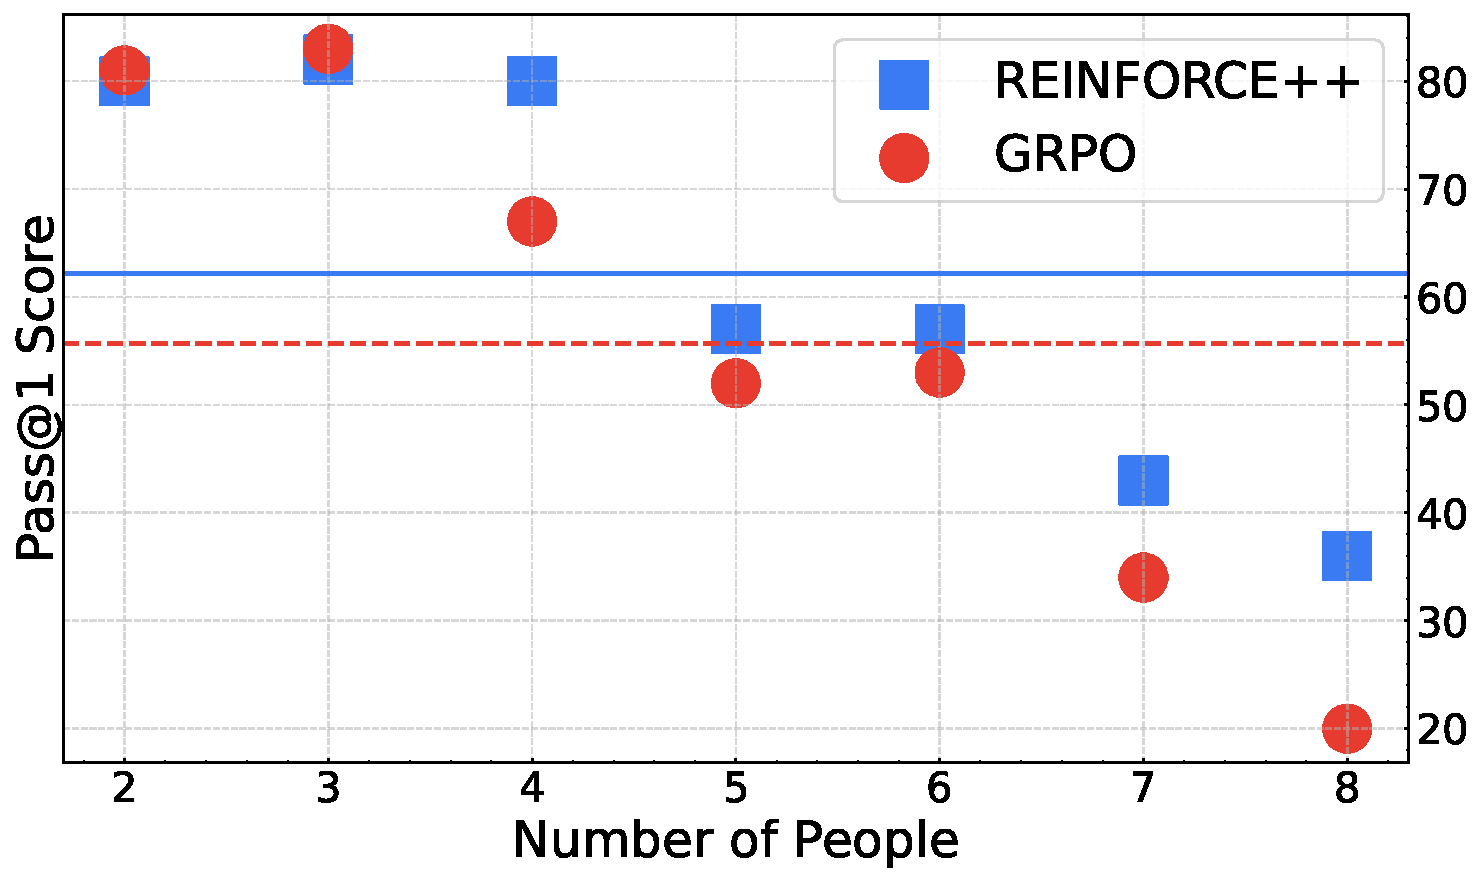
\includegraphics[width=0.76\linewidth]{imgs/logic_score.pdf}
\caption{Knights and Knaves results as the number of people increases. \ours scores higher on the evaluated tasks with at least four people, including the eight-person out-of-distribution setting.}
\label{fig:logic}
\end{figure}

\paragraph{RL from a base model.}
We also apply RL directly to a Qwen2.5-Math-Base model on MATH dataset splits. \Cref{tab:zero} reports higher scores for \ours on both out-of-distribution benchmarks: 21.04 versus 18.96 on AIME 2024 and 60.47 versus 59.22 on AMC 2023. Its MATH-500 score remains close to GRPO's (72.00 versus 73.00), extending the generalization results to RL initialized from a base model.

\begin{table}[htbp]
\caption{Reasoning results after RL from Qwen2.5-Math-Base. OOD and ID denote out-of-distribution and in-distribution evaluation relative to the training task. Scores are percentages.}
\label{tab:zero}
\centering
\begin{tabular}{lrrr}
\toprule
 & AIME 2024 (OOD) & AMC 2023 (OOD) & MATH-500 (ID) \\
Method & pass@8 & pass@8 & pass@1 \\
\midrule
GRPO & 18.96 & 59.22 & \textbf{73.00} \\
\ours & \textbf{21.04} & \textbf{60.47} & 72.00 \\
\bottomrule
\end{tabular}
\end{table}

\FloatBarrier
\subsection{Multi-step tool use}\label{sec:tools}
\paragraph{Setup.}
We use the ZeroTIR environment and its training and evaluation protocol~\citep{mai2025agentrlscalinglaw}. A Qwen2.5-7B base policy learns to call Python tools to solve mathematical problems. Training uses OpenRLHF and data from ORZ~\citep{hu2025openreasonerzeroopensourceapproach} and DAPO~\citep{yu2025dapoopensourcellmreinforcement}. Evaluation covers AIME 2024, AIME 2025, HMMT February 2024 and 2025, and CMIMC, using average@32. This metric averages success over 32 sampled attempts rather than counting success if any one attempt is correct.

\begin{table}[htbp]
\caption{Multi-step tool-use scores (average@32, in percent). ``Baseline'' denotes \baseline. The last column is the unweighted mean across the five benchmarks.}
\label{tab:tools}
\centering
\small
\begin{tabular}{lrrrrrr}
\toprule
 & \multicolumn{2}{c}{AIME} & \multicolumn{2}{c}{HMMT Feb.} & & \\
\cmidrule(lr){2-3}\cmidrule(lr){4-5}
Method & 2024 & 2025 & 2025 & 2024 & CMIMC & Mean \\
\midrule
GRPO & \textbf{31.66} & 21.87 & 16.97 & 17.70 & 24.68 & 22.58 \\
PPO & 30.20 & 21.66 & 15.00 & 18.43 & 23.95 & 21.85 \\
Baseline & 30.83 & \textbf{27.18} & \textbf{17.91} & \textbf{18.95} & \textbf{25.62} & \textbf{24.10} \\
\bottomrule
\end{tabular}
\end{table}

\paragraph{Results.}
\baseline obtains the highest mean score, 24.10, compared with 22.58 for GRPO and 21.85 for PPO (\cref{tab:tools}). It leads on four of the five benchmarks. The absolute mean improvements are 1.52 and 2.25 percentage points over GRPO and PPO, respectively. The largest gain over GRPO occurs on AIME 2025, where the score increases from 21.87 to 27.18. These results demonstrate the effectiveness of the combined training recipe for multi-step tool use.

\FloatBarrier
\section{Design implications}\label{sec:discussion}
\paragraph{A shared scale with an optional local baseline.}
The framework separates two roles that are coupled in group-standardized methods. A local baseline measures a response relative to alternatives for the same prompt. Global normalization provides a shared scale for optimization across prompts. The basic variant uses the latter without requiring grouped responses, while \baseline combines both. This separation gives a common formulation for single-response alignment and grouped reasoning or tool-use training.

\paragraph{Allocating the response budget.}
With $B$ generated responses, $k=1$ permits up to $B$ distinct prompts. Larger $k$ trades some of that prompt coverage for repeated exploration of each prompt. For leave-one-out reward centering, fixed-budget analysis identifies a trade-off between local-baseline quality, baseline-estimation noise, and the number of independent prompt draws~\citep{hu2026groupbatch}. The alignment experiment demonstrates the value of the single-response configuration, while the reasoning and tool-use experiments illustrate grouped sampling. The choice follows the task's reward structure and sampling requirements.

\paragraph{Making the optimization convention explicit.}
Normalization determines the center and scale of the advantage signal; loss reduction determines how token contributions are combined. Our batch mean loss assigns equal outer weight to each response, with token contributions averaged within that response. Stating both choices makes the method easier to implement and the reported comparisons easier to interpret.

\section{Conclusion}
\ours separates the choice of a prompt-level baseline from the scope of advantage normalization. Both variants use a shared batch scale and a clipped policy objective without training a critic. The basic variant supports single-response sampling, while \baseline combines grouped responses with a local reward baseline and separate KL regularization. Across the reported experiments, these designs provide competitive preference alignment and improvements on several held-out reasoning and tool-use benchmarks. The results identify global normalization as a useful component of critic-free post-training and motivate controlled studies of its interaction with sampling, loss reduction, and KL regularization.


\clearpage
\subsection*{AI use statement}
Generative AI tools assisted with manuscript organization, language editing, LaTeX formatting, reference checks, mathematical exposition and proof revision, and interpretation of the reported results. This assistance used the existing experimental results and did not produce new experimental measurements.

\subsection*{Reproducibility statement}
\Cref{sec:method} specifies the two algorithms, and \cref{sec:experiments} describes the experimental settings. \Cref{appendix:batch_mean} gives the loss reduction used in the experiments. \Cref{appendix:normalization,appendix:kl} provide the assumptions and derivations for the normalization and KL analyses.

\bibliographystyle{iclr2027_conference}
\bibliography{references}
\clearpage
\appendix
\section{Batch mean loss used in the experiments}\label{appendix:batch_mean}
\textbf{All experiments use a mean over valid tokens within each response, followed by a mean over responses in the batch.} This section specifies the reduction independently of advantage normalization.

Let $m_{i,t}\in\{0,1\}$ indicate a valid response token included in the policy loss, and let $n_i=\sum_t m_{i,t}>0$. For $B$ responses, the policy loss is
\begin{equation}
 \boxed{
 L_{\mathrm{PG}}(\theta)=\frac{1}{B}\sum_{i=1}^{B}
 \left[\frac{1}{n_i}\sum_t m_{i,t}\,\ell_{i,t}(\theta)\right],
 \qquad
 \ell_{i,t}(\theta)=-f_{i,t}(\theta,\sg[\widehat A_{i,t}]).
 }
 \label{eq:batch_mean}
\end{equation}
Here $f$ is the clipped surrogate in \cref{eq:clipped}, and $\sg$ denotes stop-gradient. Padding and positions outside the response loss mask do not enter the numerator or token count. The separate $k_2$ term in \cref{eq:baseline_loss} uses the same reduction.

\paragraph{Response weighting.}
Each response has outer weight $1/B$, and each valid token within response $i$ has weight $1/(Bn_i)$. This differs from dividing the sum of all token losses by the total number of valid tokens:
\begin{equation}
 L_{\mathrm{token}}=\frac{\sum_{i,t}m_{i,t}\ell_{i,t}}{\sum_i n_i}.
\end{equation}
The latter weights each response in proportion to its length. The two reductions agree when all responses have equal length. With a fixed number $k$ of responses per prompt, batch averaging is also equivalent to averaging the per-response losses within each prompt and then across prompts.

\paragraph{Minibatches and accumulation.}
For a minibatch $\mathcal M$, replace $B$ by $|\mathcal M|$ in \cref{eq:batch_mean}. To recover the same mean when combining uneven microbatches or distributed shards, their loss sums must be weighted by their response counts. The normalization moments are associated with the rollout batch; changing the partition into minibatches does not change the definition of the already computed advantages.

\paragraph{Terminal reward and token returns.}
For the basic variant, the immediate reward can be written as
\begin{equation}
 \widetilde r_{i,t}=\mathbf{1}\{t=T_i\}r(q_i,o_i)-\beta d_{i,t}.
\end{equation}
With unit discount, its return is $\sum_{u=t}^{T_i}\widetilde r_{i,u}=G_{i,t}$ from \cref{eq:return}. Thus, a terminal task reward contributes to the return at every preceding response position. For \baseline, the group-centered terminal reward in \cref{eq:group_center} is broadcast to response positions before global normalization.

\clearpage
\section{Finite-sample properties of normalization}\label{appendix:normalization}
We analyze a scalar model to make the effect of estimating normalization statistics from the same samples explicit. Let
\begin{equation}
 r_i=\mu+\epsilon_i,\qquad \epsilon_i\overset{\mathrm{i.i.d.}}{\sim}\mathcal N(0,\sigma^2),\qquad \sigma>0,
\end{equation}
and define $\bar\epsilon=N^{-1}\sum_i\epsilon_i$,
$D_N^2=N^{-1}\sum_i(\epsilon_i-\bar\epsilon)^2$, and
$Z_{i,N}=(\epsilon_i-\bar\epsilon)/D_N$ for $N\geq2$. The population-standardized target is $\epsilon_i/\sigma$. We omit the numerical stabilizer for this analysis; $D_N>0$ almost surely under the stated model.

\begin{proposition}[Finite-sample bound]\label{prop:bound}
For any nonconstant sample of size $N\geq2$, $|Z_{i,N}|\leq\sqrt{N-1}$.
Consequently, under the Gaussian model, $\E[Z_{i,N}\mid\epsilon_i]$ cannot equal $\epsilon_i/\sigma$ almost surely for finite $N$.
\end{proposition}
\begin{proof}
Set $x_j=\epsilon_j-\bar\epsilon$, so $\sum_jx_j=0$. By Cauchy--Schwarz,
\begin{equation}
 x_i^2=\left(\sum_{j\ne i}x_j\right)^2
 \leq(N-1)\sum_{j\ne i}x_j^2.
\end{equation}
Therefore $\sum_jx_j^2\geq Nx_i^2/(N-1)$, giving
$Z_{i,N}^2=Nx_i^2/\sum_jx_j^2\leq N-1$.
The conditional expectation obeys the same bound, whereas
$|\epsilon_i|/\sigma>\sqrt{N-1}$ has positive probability for a Gaussian variable. Equality with the standardized target cannot hold almost surely.
\end{proof}

\paragraph{An exact two-response example.}
For $N=2$, $D_2=|\epsilon_1-\epsilon_2|/2$ and
$Z_{1,2}=\operatorname{sign}(\epsilon_1-\epsilon_2)$ almost surely. Thus,
\begin{equation}
 \E[Z_{1,2}\mid\epsilon_1=x]=2\Phi(x/\sigma)-1,
 \label{eq:two_sample}
\end{equation}
where $\Phi$ is the standard normal cumulative distribution function. This bounded, nonlinear function differs from the linear population-standardized value $x/\sigma$. It illustrates how a small group changes the reward scale through self-normalization.

\begin{proposition}[Large-sample limit]\label{prop:limit}
Under the Gaussian model, for any fixed $i$, $Z_{i,N}\to\epsilon_i/\sigma$ almost surely and in $L^1$ as $N\to\infty$. In particular,
\begin{equation}
 \E\left[\left|\E[Z_{i,N}\mid\epsilon_i]-\epsilon_i/\sigma\right|\right]\longrightarrow0.
\end{equation}
\end{proposition}
\begin{proof}
The strong law gives $\bar\epsilon\to0$ and $D_N^2\to\sigma^2$ almost surely, establishing the first limit. By exchangeability and $\sum_{j=1}^{N}Z_{j,N}^2=N$, we have $\E[Z_{i,N}^2]=1$ for every $N$. This uniform second-moment bound implies uniform integrability, so the almost-sure convergence also holds in $L^1$. Conditional Jensen's inequality gives
\begin{equation}
 \E\left[\left|\E[Z_{i,N}-\epsilon_i/\sigma\mid\epsilon_i]\right|\right]
 \leq\E\left[|Z_{i,N}-\epsilon_i/\sigma|\right]\to0.
\end{equation}
\end{proof}

\paragraph{Implications for global normalization.}
The propositions isolate the effect of normalization sample size: estimated moments approach their population values as the number of independent observations grows. A shared batch scale can use observations across many prompt groups, rather than estimating a separate scale from each small group. For grouped or token-level data, the interpretation depends on the number of independently sampled trajectories and their dependence structure.

\paragraph{Relationship to baselines and gradients.}
For an unscaled group mean, $\E[r_i-\bar r_q\mid r_i,q]=(1-1/k)(r_i-\mu_q)$ when responses are conditionally independent with mean reward $\mu_q$. This is the same factor appearing in \cref{eq:rloo_relation}. The propositions concern convergence to a standardized scalar target, distinct from unbiasedness of a policy-gradient estimator. Their role is to explain the normalization mechanism under explicit sampling assumptions.

\clearpage
\section{KL regularization as a gradient surrogate}\label{appendix:kl}
For a fixed context, write $p_\theta(y)=\pi_\theta(y\mid h)$, $q(y)=\pi_{\mathrm{ref}}(y\mid h)$, and $z(y)=\log[p_\theta(y)/q(y)]$. Assume common support and sufficient regularity to interchange differentiation and expectation. The reverse KL is
\begin{equation}
 \KL(p_\theta\|q)=\E_{y\sim p_\theta}[z(y)],
 \qquad
 \nabla_\theta\KL(p_\theta\|q)
 =\E_{p_\theta}[z(y)\nabla_\theta\log p_\theta(y)],
 \label{eq:rkl_gradient}
\end{equation}
using $\E_{p_\theta}[\nabla_\theta\log p_\theta]=0$.

\paragraph{Value estimators and differentiated losses.}
The common expressions are
\begin{equation}
 k_1(z)=z,\qquad k_2(z)=\tfrac12 z^2,\qquad k_3(z)=e^{-z}-1+z.
\end{equation}
Both $k_1$ and $k_3$ have expectation $\KL(p_\theta\|q)$ under on-policy sampling, since $\E_{p_\theta}[e^{-z}]=1$. When sampled actions are treated as fixed during automatic differentiation, their pointwise gradients differ:
\begin{equation}
\begin{aligned}
 \nabla_\theta k_1 &=\nabla_\theta\log p_\theta,\\
 \nabla_\theta k_2 &=z\nabla_\theta\log p_\theta,\\
 \nabla_\theta k_3 &=(1-q/p_\theta)\nabla_\theta\log p_\theta.
\end{aligned}
\label{eq:kl_pointwise}
\end{equation}
The on-policy expectation of the $k_2$ pointwise gradient is exactly \cref{eq:rkl_gradient}. This is the gradient-surrogate interpretation used for the separate KL term in \baseline~\citep{liu2025rethinking}. It is distinct from differentiating the entire expectation $\E_{p_\theta}[k_2]$, which also differentiates the sampling distribution.

Under the same fixed-context assumptions, the expected pointwise gradient of $k_1$ is zero. The $k_1$ expression can instead enter the reward and act as a detached score-function coefficient, as in the returns used by the basic variant. The expected pointwise gradient of $k_3$ equals $-\E_q[\nabla_\theta\log p_\theta]$, the forward-KL gradient. Its value-estimation and loss-gradient roles should therefore be distinguished.

\paragraph{Rollout reuse.}
The on-policy identities apply when the sampled actions follow the current policy. For actions sampled from $p_{\mathrm{old}}$, a fixed-context importance-weighted gradient satisfies
\begin{equation}
 \E_{p_{\mathrm{old}}}\left[
 \frac{p_\theta(y)}{p_{\mathrm{old}}(y)}z(y)\nabla_\theta\log p_\theta(y)
 \right]=\nabla_\theta\KL(p_\theta\|q).
\end{equation}
The practical separate loss in \cref{eq:baseline_loss} is the unweighted $k_2$ surrogate on the rollout data. Its exact gradient-equivalence interpretation applies at the on-policy point; subsequent optimization uses it as a surrogate. For autoregressive policies, the fixed-context statement concerns the conditional next-token distribution.

\clearpage
\section{Additional training traces}\label{appendix:curves}
\begin{figure}[h!]
\centering
\begin{subfigure}{0.93\linewidth}
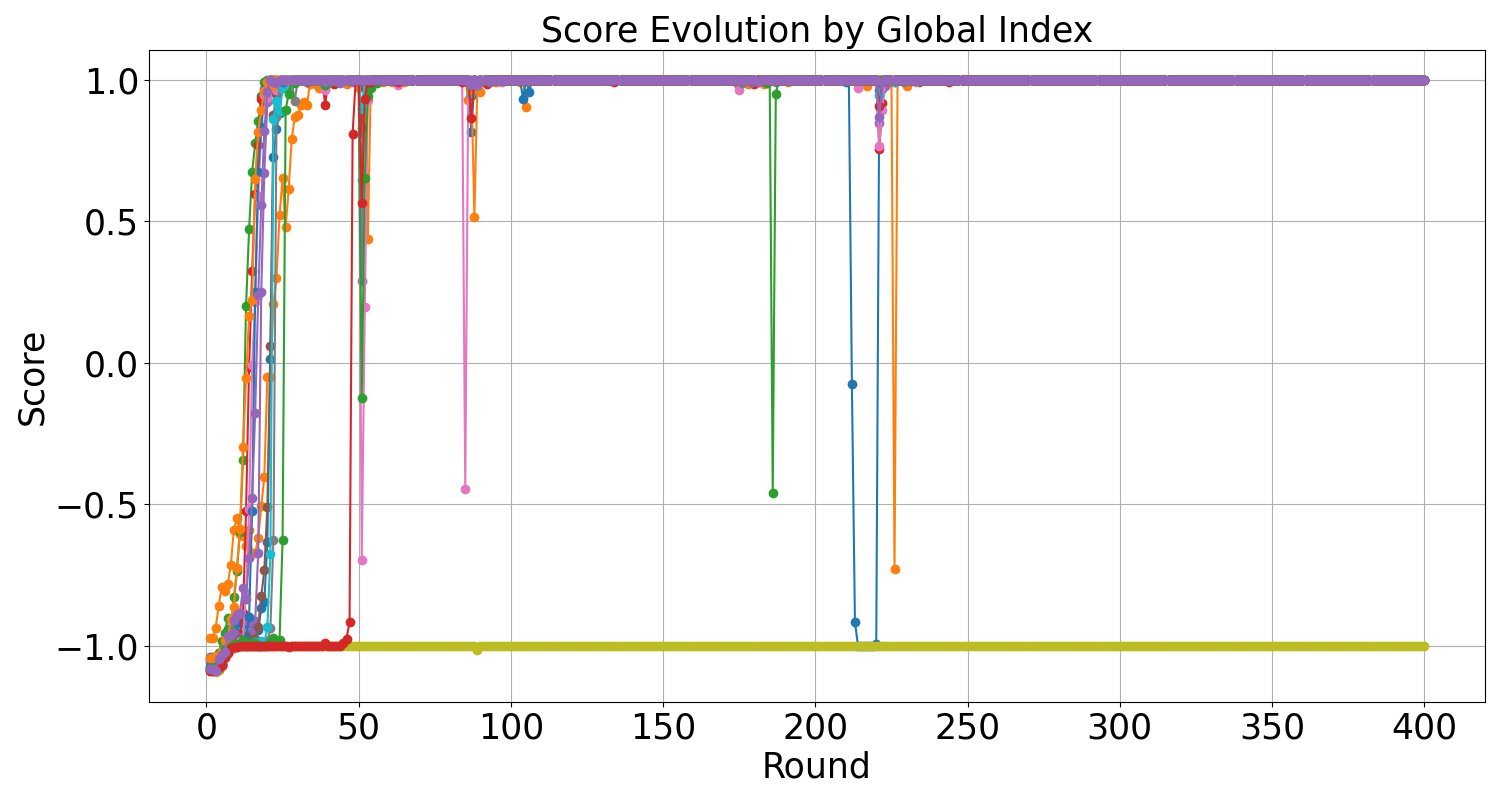
\includegraphics[width=\linewidth]{imgs/GRPO.png}
\caption{GRPO}
\end{subfigure}

\medskip
\begin{subfigure}{0.93\linewidth}
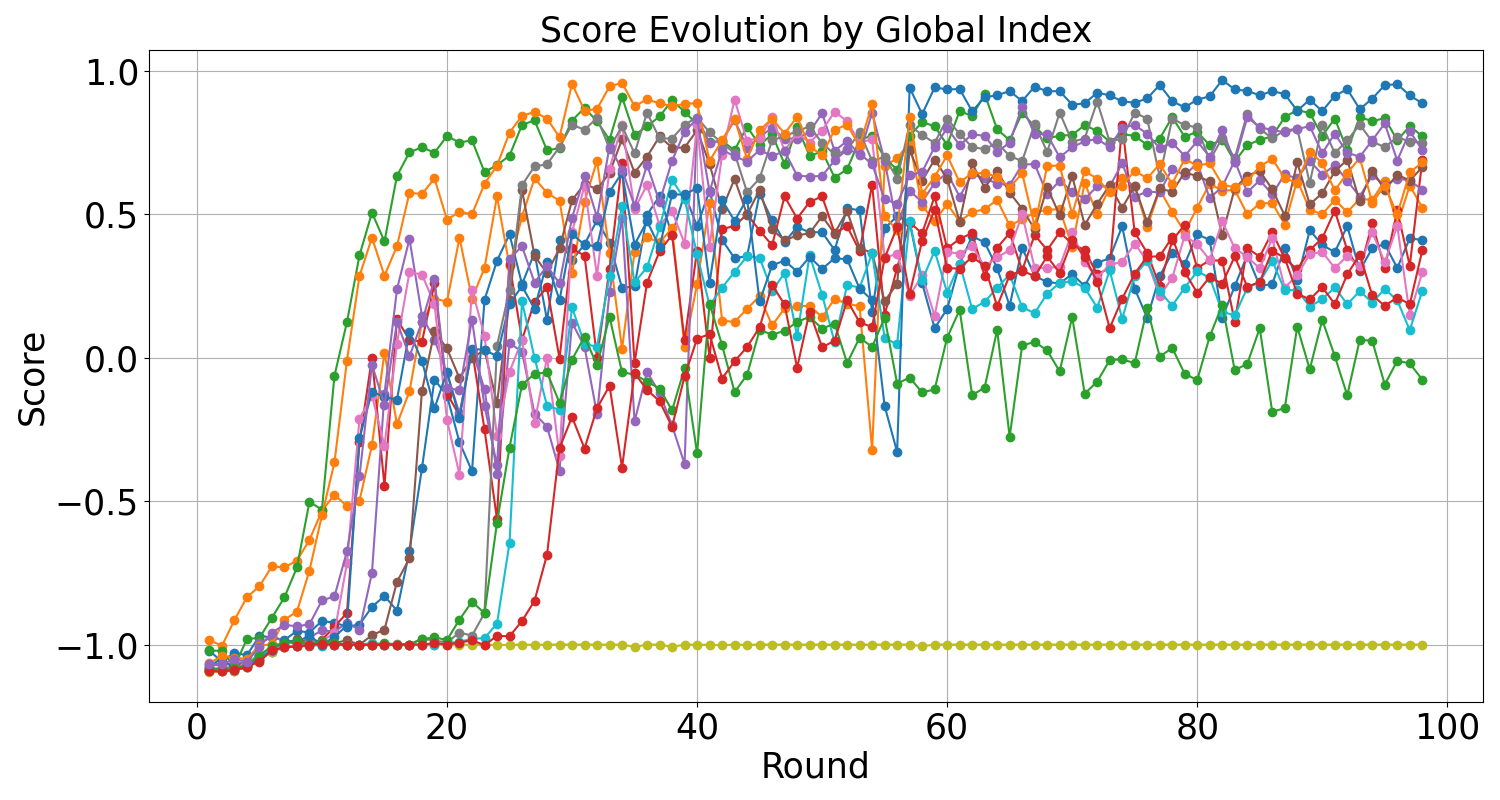
\includegraphics[width=\linewidth]{imgs/REINFORCE++.png}
\caption{REINFORCE++}
\end{subfigure}
\caption{Training traces on the small prompt set. The panels display within-run dynamics over 400 rounds for GRPO and 100 rounds for \ours.}
\label{fig:small_curves}
\end{figure}

\end{document}
